%% For double-blind review submission, w/o CCS and ACM Reference (max submission space)
\documentclass[acmsmall,review,anonymous]{acmart}\settopmatter{printfolios=true,printccs=false,printacmref=false}
%% For double-blind review submission, w/ CCS and ACM Reference
%\documentclass[acmsmall,review,anonymous]{acmart}\settopmatter{printfolios=true}
%% For single-blind review submission, w/o CCS and ACM Reference (max submission space)
%\documentclass[acmsmall,review]{acmart}\settopmatter{printfolios=true,printccs=false,printacmref=false}
%% For single-blind review submission, w/ CCS and ACM Reference
%\documentclass[acmsmall,review]{acmart}\settopmatter{printfolios=true}
%% For final camera-ready submission, w/ required CCS and ACM Reference
%\documentclass[acmsmall]{acmart}\settopmatter{}


%% Journal information
%% Supplied to authors by publisher for camera-ready submission;
%% use defaults for review submission.
\acmJournal{PACMPL}
\acmVolume{1}
\acmNumber{CONF} % CONF = POPL or ICFP or OOPSLA
\acmArticle{1}
\acmYear{2018}
\acmMonth{1}
\acmDOI{} % \acmDOI{10.1145/nnnnnnn.nnnnnnn}
\startPage{1}

%% Copyright information
%% Supplied to authors (based on authors' rights management selection;
%% see authors.acm.org) by publisher for camera-ready submission;
%% use 'none' for review submission.
\setcopyright{none}
%\setcopyright{acmcopyright}
%\setcopyright{acmlicensed}
%\setcopyright{rightsretained}
%\copyrightyear{2018}           %% If different from \acmYear

%% Bibliography style
\bibliographystyle{ACM-Reference-Format}
%% Citation style
%% Note: author/year citations are required for papers published as an
%% issue of PACMPL.
\citestyle{acmauthoryear}   %% For author/year citations


%%%%%%%%%%%%%%%%%%%%%%%%%%%%%%%%%%%%%%%%%%%%%%%%%%%%%%%%%%%%%%%%%%%%%%
%% Note: Authors migrating a paper from PACMPL format to traditional
%% SIGPLAN proceedings format must update the '\documentclass' and
%% topmatter commands above; see 'acmart-sigplanproc-template.tex'.
%%%%%%%%%%%%%%%%%%%%%%%%%%%%%%%%%%%%%%%%%%%%%%%%%%%%%%%%%%%%%%%%%%%%%%


%% Some recommended packages.
\usepackage{booktabs}   %% For formal tables:
                        %% http://ctan.org/pkg/booktabs
\usepackage{subcaption} %% For complex figures with subfigures/subcaptions
                        %% http://ctan.org/pkg/subcaption
\usepackage{catchfilebetweentags} %% For importing code snippets

%%%%%%%%%%%%%%%%%%%%%%%%%%%%%%%%%%%%%%%%%%%%%%%%%%%%%%%%%%%%%%%%%%%%%%%%%%%%%%%%
%% Agda special Characters
%%%%%%%%%%%%%%%%%%%%%%%%%%%%%%%%%%%%%%%%%%%%%%%%%%%%%%%%%%%%%%%%%%%%%%%%%%%%%%%%
\usepackage{amssymb}
\usepackage{turnstile}
\usepackage{bbm}
\usepackage[greek, english]{babel}
\usepackage{MnSymbol}
\usepackage{stmaryrd}
\usepackage{csquotes}
\newcommand\doubleplus{+\kern-1.3ex+\kern0.8ex}
\newcommand\mdoubleplus{\ensuremath{\mathbin{+\mkern-8mu+}}}
\makeatletter
\newcommand\incircbin
{%
  \mathpalette\@incircbin
}
\newcommand\@incircbin[2]
{%
  \mathbin%
  {%
    \ooalign{\hidewidth$#1#2$\hidewidth\crcr$#1\bigcirc$}%
  }%
}
\newcommand{\oeq}{\ensuremath{\incircbin{=}}}
\makeatother
\makeatletter
\newcommand\insquarebin
{%
  \mathpalette\@insquarebin
}
\newcommand\@insquarebin[2]
{%
  \mathbin%
  {%
    \ooalign{\hidewidth$#1#2$\hidewidth\crcr$#1\bigbox$}%
  }%
}
\newcommand{\sqtri}{\ensuremath{\insquarebin{\triangle}}}
\makeatother
\usepackage{ucs}
\DeclareUnicodeCharacter{8759}{\ensuremath{\squaredots}}
\DeclareUnicodeCharacter{951}{\textgreek{\texteta}}
\DeclareUnicodeCharacter{737}{\ensuremath{^\text{l}}}
\DeclareUnicodeCharacter{691}{\ensuremath{^\text{r}}}
\DeclareUnicodeCharacter{7523}{\ensuremath{_\text{r}}}
\DeclareUnicodeCharacter{8718}{\ensuremath{\blacksquare}}
\DeclareUnicodeCharacter{957}{\textgreek{\textnu}}
\DeclareUnicodeCharacter{961}{\textgreek{\textrho}}
\DeclareUnicodeCharacter{929}{\textgreek{\textRho}}
\DeclareUnicodeCharacter{954}{\textgreek{\textkappa}}
\DeclareUnicodeCharacter{10214}{\ensuremath{\lsem}}
\DeclareUnicodeCharacter{10215}{\ensuremath{\rsem}}
\DeclareUnicodeCharacter{8857}{\mdoubleplus}
\DeclareUnicodeCharacter{8860}{\oeq}
\DeclareUnicodeCharacter{9043}{\ensuremath{\sqtri}}
\DeclareUnicodeCharacter{928}{\textgreek{\textPi}}
\DeclareUnicodeCharacter{922}{\textgreek{\textKappa}}
\DeclareUnicodeCharacter{931}{\textgreek{\textSigma}}
\DeclareUnicodeCharacter{916}{\textgreek{\textDelta}}
\DeclareUnicodeCharacter{921}{\textgreek{\textIota}}
\DeclareUnicodeCharacter{8779}{\ensuremath{\backtriplesim}}
\DeclareUnicodeCharacter{8799}{\ensuremath{\stackrel{?}{=}}}
\DeclareUnicodeCharacter{10181}{\ensuremath{\lbag}}
\DeclareUnicodeCharacter{10182}{\ensuremath{\rbag}}
\DeclareUnicodeCharacter{8760}{\ensuremath{-}}
\usepackage[references]{agda}
%%%%%%%%%%%%%%%%%%%%%%%%%%%%%%%%%%%%%%%%%%%%%%%%%%%%%%%%%%%%%%%%%%%%%%%%%%%%%%%%


\begin{document}

%% Title information
\title[Reading and Writing Arithmetic]{Reading and Writing Arithmetic: Automating Ring Equalities
  in Agda}

%% Author information
%% Contents and number of authors suppressed with 'anonymous'.
%% Each author should be introduced by \author, followed by
%% \authornote (optional), \orcid (optional), \affiliation, and
%% \email.
%% An author may have multiple affiliations and/or emails; repeat the
%% appropriate command.
%% Many elements are not rendered, but should be provided for metadata
%% extraction tools.

%% Author with single affiliation.
\author{Donnacha Oisín Kidney}
\authornote{with author1 note}          %% \authornote is optional;
                                        %% can be repeated if necessary
\orcid{nnnn-nnnn-nnnn-nnnn}             %% \orcid is optional
\affiliation{
  \position{Position1}
  \department{Department1}              %% \department is recommended
  \institution{Institution1}            %% \institution is required
  \streetaddress{Street1 Address1}
  \city{City1}
  \state{State1}
  \postcode{Post-Code1}
  \country{Country1}                    %% \country is recommended
}
\email{first1.last1@inst1.edu}          %% \email is recommended

%% Author with two affiliations and emails.
\author{First2 Last2}
\authornote{with author2 note}          %% \authornote is optional;
                                        %% can be repeated if necessary
\orcid{nnnn-nnnn-nnnn-nnnn}             %% \orcid is optional
\affiliation{
  \position{Position2a}
  \department{Department2a}             %% \department is recommended
  \institution{Institution2a}           %% \institution is required
  \streetaddress{Street2a Address2a}
  \city{City2a}
  \state{State2a}
  \postcode{Post-Code2a}
  \country{Country2a}                   %% \country is recommended
}
\email{first2.last2@inst2a.com}         %% \email is recommended
\affiliation{
  \position{Position2b}
  \department{Department2b}             %% \department is recommended
  \institution{Institution2b}           %% \institution is required
  \streetaddress{Street3b Address2b}
  \city{City2b}
  \state{State2b}
  \postcode{Post-Code2b}
  \country{Country2b}                   %% \country is recommended
}
\email{first2.last2@inst2b.org}         %% \email is recommended



%% Abstract
%% Note: \begin{abstract}...\end{abstract} environment must come
%% before \maketitle command
\begin{abstract}
  We present a new library which automates the construction of equivalence
  proofs between polynomials over commutative rings and semirings in the
  programming language Agda \cite{norell_dependently_2008}. It is asymptotically
  faster than Agda's existing solver. We use reflection to provide a simple
  interface to the solver, and demonstrate a novel use of the constructed
  relations: step-by-step solutions.
\end{abstract}


%% 2012 ACM Computing Classification System (CSS) concepts
%% Generate at 'http://dl.acm.org/ccs/ccs.cfm'.
\begin{CCSXML}
<ccs2012>
<concept>
<concept_id>10011007.10011006.10011008</concept_id>
<concept_desc>Software and its engineering~General programming languages</concept_desc>
<concept_significance>500</concept_significance>
</concept>
<concept>
<concept_id>10003456.10003457.10003521.10003525</concept_id>
<concept_desc>Social and professional topics~History of programming languages</concept_desc>
<concept_significance>300</concept_significance>
</concept>
</ccs2012>
\end{CCSXML}

\ccsdesc[500]{Software and its engineering~General programming languages}
\ccsdesc[300]{Social and professional topics~History of programming languages}
%% End of generated code


%% Keywords
%% comma separated list
\keywords{proof automation, equivalence, proof by reflection, step-by-step solutions}


%% \maketitle
%% Note: \maketitle command must come after title commands, author
%% commands, abstract environment, Computing Classification System
%% environment and commands, and keywords command.
\maketitle

\begin{figure}[h]
  \begin{subfigure}[b]{\linewidth}
    \centering
    \ExecuteMetaData[../Introduction.tex]{lemma}
    \label{ring-lemma}
  \end{subfigure}
  \begin{subfigure}[b]{.5\linewidth}
    \ExecuteMetaData[../Introduction.tex]{proof}
    \caption{A Tedious Proof}
    \label{ring-proof}
  \end{subfigure}%
  \begin{subfigure}[b]{.3\linewidth}
    \centering
    \ExecuteMetaData[../Introduction.tex]{solver}
    \caption{The Solver}
    \label{the-solver}
  \end{subfigure}
  \caption{Comparison Between A Manual Proof and The Automated Solver}
  \label{comparison}
\end{figure}

\begin{figure}
  \ExecuteMetaData[../Introduction.tex]{old-solver}
  \caption{The Old Solver}
  \label{old-solver}
\end{figure}
\section{Introduction}
Doing mathematics in dependently-typed programming languages like Agda has a
reputation for being tedious, awkward, and difficult. Even simple arithmetic
identities like the one in Fig.~\ref{comparison} require fussy proofs
(Fig.~\ref{ring-proof}).

This need not be the case! With some carefully-designed tools, mathematics in
Agda can be easy, friendly, and fun. This work describes one such tool: an
Agda library which automates the construction of these kinds of proofs, making
them as easy as Fig.~\ref{the-solver}.

As you might expect, our solver comes accompanied by a formal proof of
correctness. Beyond that, though, we also strove to satisfy the following
requirements:
\begin{description}
  \item[Friendliness and Ease of Use] Proofs like the one in
    Fig.~\ref{ring-proof} aren't just boring: they're \emph{difficult}.
    The programmer needs to remember the particular syntax for each step (``is
    it \(\AgdaFunction{+-comm}\) or \(\AgdaFunction{+-commutative}\)?''), and
    often they have to put up with poor error messages.

    We believe this kind of difficulty is why Agda's current ring solver
    \cite{danielsson_agda_2018} enjoys little widespread use. Its interface
    (Fig.~\ref{old-solver}) is almost as verbose as the manual proof, and it
    requires programmers to learn another syntax specific to the solver.

    Our solver strives to be as easy to use as possible: the high-level
    interface is simple (Fig.~\ref{the-solver}), we don't require anything
    of the user other than an implementation of one of the supported algebras,
    and effort is made to generate useful error messages.
  \item[Performance] Typechecking dependently-typed code is a costly task.
    Automated solvers like the one presented here can greatly exacerbate this
    cost: in our experience, it wasn't uncommon for Agda's current ring solver
    to spend upwards of 10 minutes proving a single identity.

    In practice, this means two things: firstly, large libraries for formalizing
    mathematics (like \citet{meshveliani_docon-provable_2018}) can potentially
    take hours to typecheck (by which time the programmer has understandably
    begun to reconsider the whole notion of mathematics on a computer);
    secondly, certain identities can simply take too long to typecheck,
    effectively making them ``unprovable'' in Agda altogether!

    The kind of solver we provide here is based on Coq's
    \cite{the_coq_development_team_2018_1219885} \verb+ring+ tactic, described
    in \citet{gregoire_proving_2005}. While we were able to apply the same
    optimizations that were applied in that paper, we found that the most
    significant performance improvements came from a different, and somewhat
    surprising part of the program. The end result is that our solver is
    asymptotically (and practically) faster than Agda's current solver.
  \item[Educational Features] While our solver comes with the benefit of formal
    correctness, it's still playing catch-up to other less-rigorous computer
    algebra systems in terms of features. These features have driven systems
    like Wolfram|Alpha \cite{wolfram_research_inc._wolframalpha_2019} to
    widespread popularity among (for instance) students learning mathematics.

    We will take just one of those features (``pedagogical'', or step-by-step
    solutions \cite{the_development_team_step-by-step_2009}), and reimplement it
    in Agda using our solver. In doing so, we will explore some of the theory
    behind it, and present a formalism that describes the nature of
    ``step-by-step'' solutions.
\end{description}

\section{Overview of the Proof Technique}
There are a number of ways we can automate proofs in a dependently-typed
programming language, including Prolog-like proof search \cite{kokke_auto_2015},
Cooper's algorithm over Presburger arithmetic \cite{allais_deciding_2011}, etc.
Here, we will use a reflexive technique \cite{boutin_using_1997} in combination
with sparse Horner Normal Form. The high-level diagram of the proof strategy is
presented in Fig.~\ref{proof-process}.

\begin{figure}
  \resizebox{\textwidth}{!}{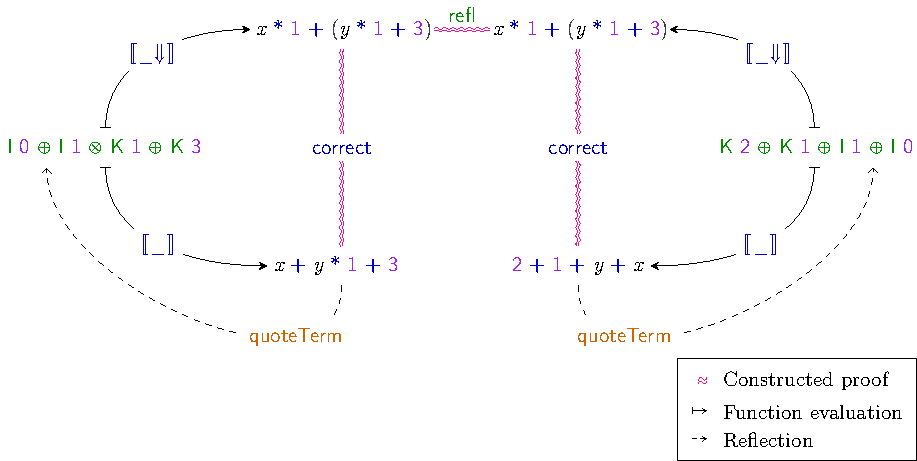
\includegraphics[draft=false]{graphics/reflexive-process}}
  \vspace*{-50pt}
  \caption{The Reflexive Proof Process}
  \label{proof-process}
\end{figure}

The identity we'll be working with is the lemma in Fig.~\ref{comparison}: the
left and right hand side of the equality are at the bottom of the diagram. Our
objective is to link those two expressions up through repeated application of
the ring axioms. We do this by converting both expressions to a normal form
(seen at the top of the diagram), and then providing a proof that this
conversion is correct according to the ring axioms (the
\(\AgdaFunction{correct}\) function in the diagram). Finally, we link up all of
these proofs, and if the two normal forms are definitionally equal, the entire
thing will typecheck, and we will have proven the equality.
\subsection{The \(\AgdaDatatype{Expr}\) AST}
In Agda, we can't manipulate the expressions we want to prove directly: instead,
we will construct an AST for each expression, and then do our manipulation on
that.

The AST type (\(\AgdaDatatype{Expr}\)) has a constructor for each of the ring
operators, as well as constructors for both variables and constants. The ASTs
for both expressions we want to prove can be seen on either side of
Fig.~\ref{proof-process}. Constants are constructed with
\(\AgdaInductiveConstructor{K}\), and variables are referred to by their de
Bruijn index (so \(x\) becomes \(\AgdaInductiveConstructor{I} \;
\AgdaNumber{0}\)).

From here, we can ``evaluate'' the AST in one of two ways: in a non-normalized
way (\(\AgdaFunction{⟦\_⟧}\)), or in a normalizing way
(\(\AgdaFunction{⟦\_⇓⟧}\)). This means that the goal of the
\(\AgdaFunction{correct}\) function is to show equivalence between
\(\AgdaFunction{⟦\_⟧}\) and \(\AgdaFunction{⟦\_⇓⟧}\).

Finally, we \emph{don't} want to force users to construct the
\(\AgdaDatatype{Expr}\) AST themselves. This is where reflection comes in: it
automates this construction (the path labeled \(\AgdaKeyword{quoteTerm}\) in the
diagram) from the goal type.
\subsection{Choice of Algebra}
So far, we have been intentionally vague about the precise algebra we're using.
As in \cite{gregoire_proving_2005}, we use an algebra called an
\emph{almost-ring}. It has the regular operations (\(+\), \(*\)
(multiplication), \(-\), \(0\), and \(1\)), such that the following equations
hold:
\begin{align}
  0 + x       &= x \\
  x + y       &= y + x \\
  x + (y + z) &= (x + y) + z \\
  1 * x       &= x \\
  x * y       &= y * x \\
  x * (y * z) &= (x * y) * z \\
  (x + y) * z &= x * z + y * z \\
  0 * x       &= 0 \label{semiring} \\
  -(x * y)    &= - x * y \label{ringmul} \\
  -(x + y)    &= -x + -y \label{ringadd}
\end{align}
The equations up to \ref{semiring} represent a pretty standard definition of a
(commutative) semiring. To get from there to a ring, we would usually ask for
something like:
\begin{align}
  x + - x = 0
\end{align}
So why do we instead ask for \ref{ringmul} and \ref{ringadd}? 

Under this formulation, we can admit types like \(\AgdaDatatype{ℕ}\) which don't
have additive inverses. Instead, these types can simply supply the identity
function for \(-\), and then \ref{ringmul} and \ref{ringadd} will still hold.

A potential worry is that because we don't require \(x + -x = 0\) axiomatically,
it won't be provable in our system. Happily, this is not the case: as long as
\(1 + -1\) reduces to \(0\) in the coefficient set, the solver will verify the
identity.
\section{The Interface}
\section{Performance}
\section{Pedagogical Proofs}
\section{Related Work}

%% Acknowledgments
\begin{acks}                            %% acks environment is optional
                                        %% contents suppressed with 'anonymous'
  %% Commands \grantsponsor{<sponsorID>}{<name>}{<url>} and
  %% \grantnum[<url>]{<sponsorID>}{<number>} should be used to
  %% acknowledge financial support and will be used by metadata
  %% extraction tools.
  This material is based upon work supported by the
  \grantsponsor{GS100000001}{National Science
    Foundation}{http://dx.doi.org/10.13039/100000001} under Grant
  No.~\grantnum{GS100000001}{nnnnnnn} and Grant
  No.~\grantnum{GS100000001}{mmmmmmm}.  Any opinions, findings, and
  conclusions or recommendations expressed in this material are those
  of the author and do not necessarily reflect the views of the
  National Science Foundation.
\end{acks}


%% Bibliography
\bibliography{../bibliography.bib}
%% Appendix
\appendix
\section{Appendix}

Text of appendix \ldots

\end{document}
